\documentclass{article}
\usepackage[utf8]{inputenc}
\usepackage{natbib}
\usepackage{graphicx}
\usepackage{caption}
\usepackage{ragged2e}
\usepackage{amsmath}
\usepackage{cancel}
\usepackage[
  a4paper, twoside,
  layout=b5paper,
  left=1cm, right=1cm, bottom=0cm, top=1cm,
  columnsep=1cm,
]{geometry}


\title{RoboticsCheatSheet}
\author{ohad-i}
\date{September 2022}

\begin{document}

%\maketitle
%\newpage
\section{Pose Description}
Pose: position and orientation
\begin{figure}[h!]
\centering
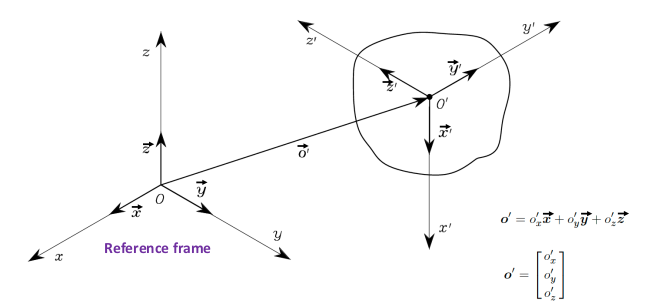
\includegraphics[scale=1.5]{pose.png}
\caption{pose smaple}
\label{fig:sr}
\end{figure}

We can desctibe the new frame (') with the following projection:

 $$\vec{x}{'}= x{'}_{x}\vec{X} + x{'}_{y}\vec{Y}  + x{'}_{z}\vec{Z}$$
 $$\vec{y}{'}= y{'}_{x}\vec{X} + y{'}_{y}\vec{Y}  + y{'}_{z}\vec{Z}$$
 $$\vec{z}{'}= z{'}_{x}\vec{X} + z{'}_{y}\vec{Y}  + z{'}_{z}\vec{Z}$$

It describes the (') frame completely.

\subsection{Rotation Matrix}

\begin{gather}
    R =
        \begin{bmatrix}
        \\
        X{'} & Y{'} & Z{'} \\
        \\
        \end{bmatrix} =
        \begin{bmatrix}
        x_{x}^{'} & y_{x}^{'} & z_{x}^{'}\\
        x_{y}^{'} & y_{y}^{'} & z_{y}^{'}\\
        x_{z}^{'} & y_{z}^{'} & z_{z}^{'}
        \end{bmatrix} =
        \begin{bmatrix}
         x{'}_{x}\vec{X} & x{'}_{y}\vec{Y}  & x{'}_{z}\vec{Z}\\
         y{'}_{x}\vec{X} & y{'}_{y}\vec{Y}  & y{'}_{z}\vec{Z}\\
         z{'}_{x}\vec{X} & z{'}_{y}\vec{Y}  & z{'}_{z}\vec{Z}
    \end{bmatrix}
\end{gather}
reminder:\\
$$ \vec{x}{'^T}\vec{y}{'} = 0 \qquad \vec{y}{'^T}\vec{z}{'} = 0 \qquad  \vec{z}{'^T}\vec{x}{'} = 0$$
$$ \vec{x}{'^T}\vec{x}{'} = 1 \qquad \vec{y}{'^T}\vec{y}{'} = 1 \qquad  \vec{z}{'^T}\vec{z}{'} = 1$$
\\
therefore, rotation matrix properties:
$$ R{^T}R=I$$
$$ R{^T}=R{^{-1}}$$
$$ |\det({R})|=1 $$
$$ R\in SO(m) $$

Special Orthonormal group: real m×m matrices with orthonormal columns and
determinant=1

 \newpage
 \subsection{Rotation along the axis - Elementry Rotations}
 \begin{figure}[h!]
\centering
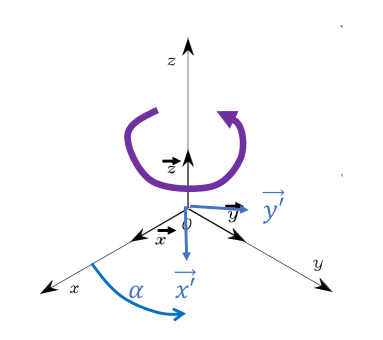
\includegraphics[scale=1.5]{rotation.png}
\caption{Rotation along z axis}
\label{fig:sr}
\end{figure}
Rotation matrices
\begin{gather}
    R_{z}(\alpha) =
    \begin{bmatrix}
    \cos\alpha & -\sin\alpha & 0 \\
    \sin\alpha & \cos\alpha & 0 \\
    0 & 0 & 1
    \end{bmatrix}
\end{gather}

\begin{gather}
    R_{y}(\beta) =
    \begin{bmatrix}
    \cos\beta & 0 & \sin\beta  \\
    0 & 1 & 0 \\
    -\sin\beta & 0 & \cos\beta
    \end{bmatrix}
\end{gather}

\begin{gather}
    R_{x}(\gamma) =
    \begin{bmatrix}
    1 & 0 & 0 \\
    0 & \cos\gamma & -\sin\gamma \\
    0 & \sin\gamma & \cos\gamma
    \end{bmatrix}
\end{gather}
Rotation in the "opposite" direction is equivalent to the inverse $ R $ matrix which is the transpose rotation matrix:
$$ R_{k}(-\vartheta) = \{R^{-1}_{k}(\vartheta)\} = R^{T}_{k}(\vartheta) \quad ; \quad k=x,y,z$$
(*) see rotation matrix properties


\newpage
\subsection{Representation of a vector}
\begin{figure}[h!]
\centering
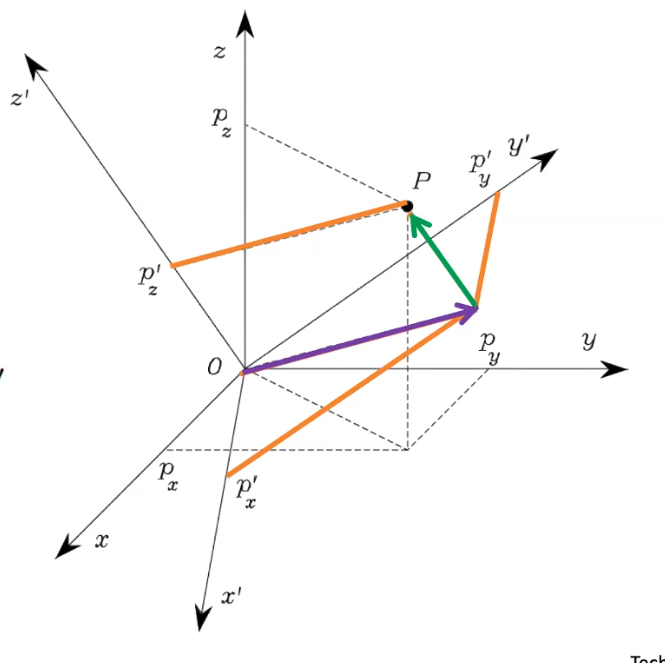
\includegraphics[scale=1.5]{vectorRep.png}
\caption{vector representation}
\label{fig:sr}
\end{figure}
$$ o^{'}=O $$
$$
P=\begin{bmatrix}
p_{x}\\ p_{y}\\ p_{z}
\end{bmatrix}
\quad
P^{'}=\begin{bmatrix}
p{'}_x\\ p{'}_y\\ p{'}_z
\end{bmatrix}
$$

$$ P = p'_{x}x'+p'_{y}y'+p'_{z}z' =
\begin{bmatrix}
\\
x' & y' & z'\\
\\
\end{bmatrix} p'$$
 $$ p=Rp' $$
 $$ p'=R^{T}p $$

$R$ Matrix represents:
\begin{enumerate}
    \item The orientation of $O'$ w.r.t $O$
    \item The transformation of vector from $O'$ to $ O$
    \item Rotation of a vector (in the same frame)
\end{enumerate}

\newpage
\subsection{Composition of Rotation matrices}
\begin{figure}[h!]
\centering
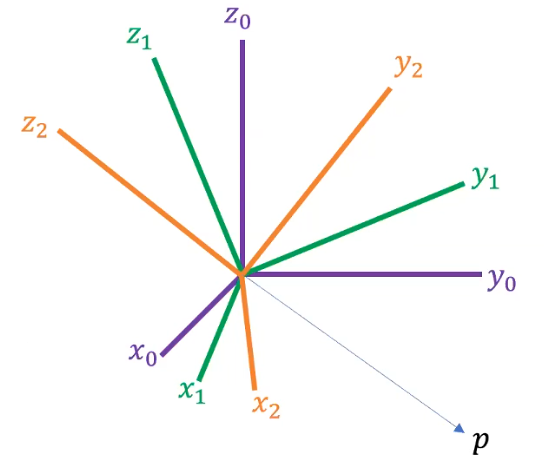
\includegraphics[scale=1.5]{compR.png}
\caption{composition}
\label{fig:sr}
\end{figure}
\begin{itemize}
    \item Consider 3 frames with same origin
    \item A point represented in each frame: $p^{0},p^{1},p^{2}$
\end{itemize}
Transformation of $O_{2}$ w.r.t $ O_{1}$: $p^{1} = R^{1}_{2}p^{2}$

$$ p^{0} = R^{0}_{1}p^{1}$$
$$ p^{0} = R^{0}_{2}p^{2} \quad \implies \quad R^{0}_{2}=R^{0}_{1}R^{1}_{2} $$
(*) from left to right from 0 to 1 and than from 1 to 2 - "current frame" method\\

we can transform from $0$ to $2$ in two steps:
\begin{itemize}

    \item First rotate the given frame according to $R^{0}_{1}$, so as to align it with frame $O_{x_{1}y_{1}z_{1}}$
    \item Then rotate the frame, now aligned with frame $O_{x_{1}y_{1}z_{1}}$ according to $R^{1}_{2}$ so as to align it with frame $O_{x_{2}y_{2}z_{2}}$
\end{itemize}

\textbf{The order matters - rotation transformation do not cummute!}\\

So we can see that we can reverse the transformation using:
$$R^{j}_{i}=(R^{i}_{j})^{-1}=(R^{j}_{i})^{T} $$

\subsection{Composition Current Frame vs. Fixed Frame}
\begin{itemize}
    \item \textbf{Current Frame} Consider the following sequence of rotations:
    \begin{enumerate}
        \item Rotate around $z_0$
        \item Rotate around $x_1$
    \end{enumerate}
    \begin{figure}[h!]
    \centering
    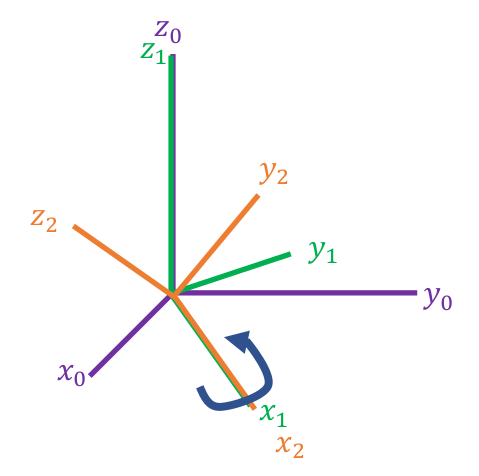
\includegraphics[scale=1.5]{currentFrame.png}
    \caption{composition}
    \label{fig:sr}
    \end{figure}

    \item \textbf{Fixed Frame} Consider the following sequence of rotations:
    \begin{enumerate}
        \item Rotate around $z_0$
        \item Rotate around $x_0$
    \end{enumerate}
    \begin{figure}[h!]
    \centering
    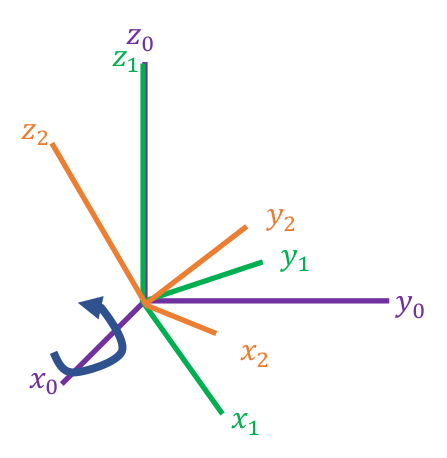
\includegraphics[scale=1.5]{fixedFrame.png}
    \caption{composition}
    \label{fig:sr}
    \end{figure}
\end{itemize}
It is obvious that the rotation gives us different rotation (current vs. fixed)\\
\textbf{We cant use the same formula!}

\subsection{Fixed Frame}
Define:
\begin{itemize}
    \item $R^{0}_1$: rotation for $O_1$ w.r.t $O_0$
    \item $R$: rotation of $O_1$ w.r.t $O_0$ to obtain $O_2$
\end{itemize}

$R^{0}_2 = R^{0}_1 R^{1}_2$: rotation for $O_2$ w.r.t $O_0$ but we know it is nto the transformation we want so... $$R^{0}_2 \ne R^{0}_1 R$$

What we really want is:\\
$$R^{0}_2 = R^{0}_1\begin{bmatrix}
(R^{0}_1)^{-1}RR^{0}_{1}
\end{bmatrix}  $$

after opening the brackets:
$\left[ R^{0}_1(R^{0}_1)^{-1} = R^{0}_1(R^{0}_1)^{T} = I \right] $

$$R^{0}_2 = RR^{0}_{1}  $$

Fix frame recipe:
\begin{enumerate}
    \item Rotate $O_1$ to align with $O_0$
    \item Apply R (by definition)
    \item Undo the rotation in (1)
\end{enumerate}

\textbf{For rotation w.r.t fixed-frame - multiply the rotation matrices in reverse order!}

\section{Parameterization of rotations}
\begin{itemize}
    \item Rotaion matrix has 9 elements
    \item The minimum parameters needed to define arbitrary rotation - 3
    \item there are several parameterization options.
\end{itemize}
\subsection{Euler angles}
\begin{itemize}
    \item Eulre angles $(ZYZ) (\phi, \theta,\psi)$
    \begin{enumerate}
        \item Rotate about Z axis by an angle $\phi, \quad R_z(\phi)$
        \item Rotate about \textbf{current} $y$ axis by an angle $\theta,  \quad R_y(\theta)$
        \item Rotate about \textbf{current} $z$ axis by an angle $\psi,  \quad R_z(\psi)$
    \begin{figure}[h!]
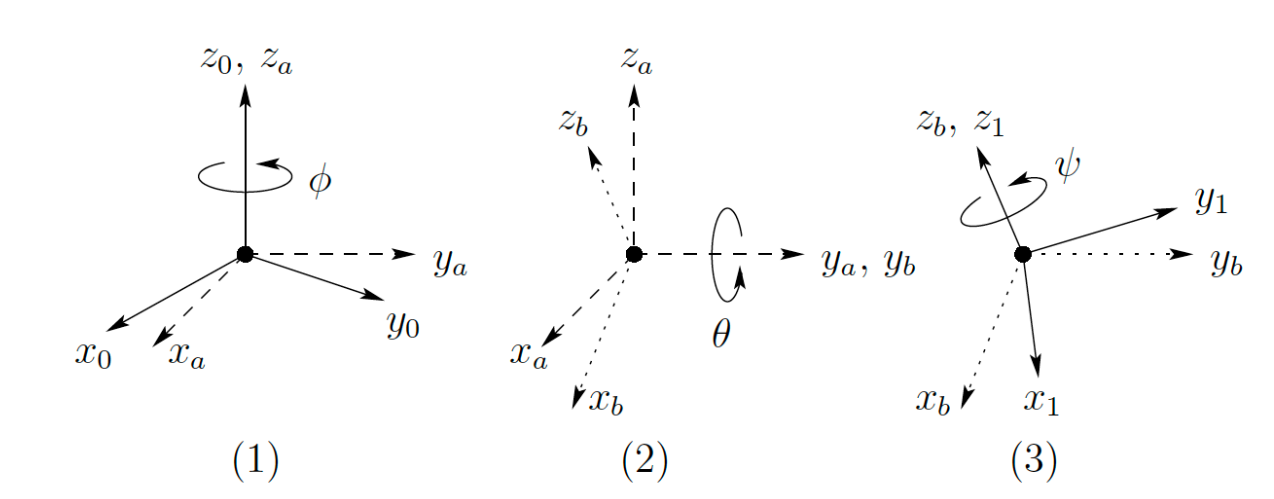
\includegraphics[scale=1.5]{euler.png}
\caption{Eulre angles $(\phi, \theta,\psi)$}
\label{fig:sr}
\centering
\end{figure}

 \begin{multline*}
    R^{0}_{1} = R_{z,\phi}R_{y,\theta}R_{z,\psi} =
    \begin{bmatrix}
    C_\phi & -S_\phi & 0 \\
    S_\phi & C_\phi & -0 \\
    0 & 0 & 1
    \end{bmatrix}
    \begin{bmatrix}
    C_\theta & 0 & S_\theta \\
    0 & 1 & 0 \\
    -S_\theta & 0 & C_\theta
    \end{bmatrix}
    \begin{bmatrix}
    C_\psi & -S_\psi &  0 \\
    S_\psi & C_\psi & 0\\
    0 & 0 & 1 \\
    \end{bmatrix} =\\ =
    \linebreak
    \begin{bmatrix}
    C_\phi C_\theta C_\psi - S_\phi S_\psi  & -C_\phi C_\theta S_\psi - S_\phi C_\psi & C_\phi S_\theta \\
    S_\phi C_\theta  C_\psi + C_\phi S_\psi & -S_\phi C_\theta  S_\psi + C_\phi C_\psi & S_\phi S_\theta \\
    -S_\theta C_\psi & S_\theta S_\psi & C_\theta
    \end{bmatrix}
 \end{multline*}

 \item Roll-Pitch-yaw (fixed frame) angles: $(\phi, \theta, \psi)$
 \begin{itemize}
     \item Rotate about \textbf{fixed} $x$ axis by an angle $\phi, \quad R_{x}(\phi)$
     \item Rotate about \textbf{fixed} $y$ axis by an angle $\theta, \quad R_{y}(\theta)$
     \item Rotate about \textbf{fixed} $z$ axis by an angle $\psi, \quad R_{z}(\psi)$ \\
(*) Fixed frame(!) multiply in reverse order.
    \begin{figure}[h!]
    \centering
    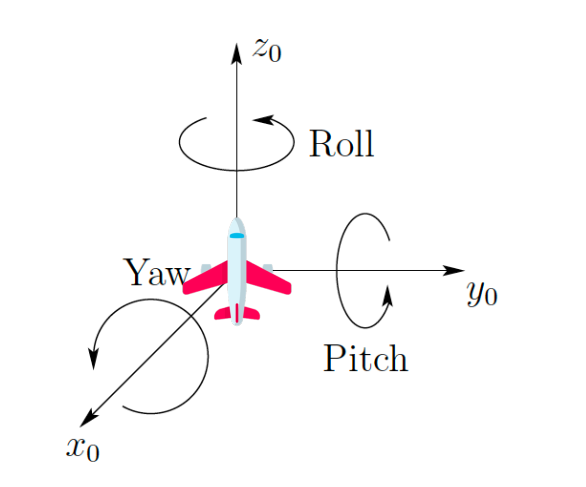
\includegraphics[scale=1.5]{rollPitchYaw.png}
    \caption{roll-pitch-yaw (bad axis tags... usually the $x$ axis is along the heading of the plane) $(\phi, \theta,\psi)$}
    \label{fig:sr}
    \end{figure}

    \begin{multline*}
    R^{0}_{1} = R_{z,\phi}R_{y,\theta}R_{x,\psi} =
    \begin{bmatrix}
    C_\phi & -S_\phi & 0 \\
    S_\phi & C_\phi & -0 \\
    0 & 0 & 1
    \end{bmatrix}
    \begin{bmatrix}
    C_\theta & 0 & S_\theta \\
    0 & 1 & 0 \\
    -S_\theta & 0 & C_\theta
    \end{bmatrix}
    \begin{bmatrix}
    1 & 0 & 0 \\
    0& C_\psi & -S_\psi \\
    0 & S_\psi & C_\psi
    \end{bmatrix} =\\ =
    \linebreak
    \begin{bmatrix}
    C_\phi C_\theta & -S_\phi C_\psi + C_\phi S_\theta S_\psi & S_\phi S_\psi + C_\phi S_\theta C_\psi \\
    S_\phi C_\theta & C_\phi C_\psi + S_\phi S_\theta S_\psi & -C_\phi S_\psi + S_\phi S_\theta C_\psi \\
    -S_\theta & C_\theta S_\psi & C_\theta C\psi
    \end{bmatrix}
 \end{multline*}
    \end{itemize}
    \end{enumerate}
\end{itemize}
\subsubsection{Euler angles - inverse problem}
    \begin{enumerate}
        \item Rotate about \textbf{fixed} $x$ by an angle $\phi$
        \item Rotate about \textbf{fixed} $y$ by an angle $\theta$
        \item Rotate about \textbf{fixed} $z$ by an angle $\psi$\\
        $$ R =
        \begin{bmatrix}
        r_{11} & r_{12} & r_{13} \\
        r_{21} & r_{22} & r_{23} \\
        r_{31} & r_{32} & r_{33}
        \end{bmatrix} \xrightarrow[]{} { (\phi,  \theta, \psi) }
        $$
        $$
        R =
        \begin{bmatrix}
        r_{11} & r_{12} & r_{13} \\
        r_{21} & r_{22} & r_{23} \\
        r_{31} & r_{32} & r_{33}
        \end{bmatrix} =
        \begin{bmatrix}
        C_\phi C_\theta & -S_\phi C_\psi + C_\phi S_\theta S_\psi & S_\phi S_\psi + C_\phi S_\theta C_\psi \\
        S_\phi C_\theta & C_\phi C_\psi + S_\phi S_\theta S_\psi & -C_\phi S_\psi + S_\phi S_\theta C_\psi \\
        -S_\theta & C_\theta S_\psi & C_\theta C\psi
        \end{bmatrix}
    $$
    \begin{equation}
    \begin{cases}
         C_\theta S_\psi = r_{32} \\
         C_\theta C_\psi = r_{13}
    \end{cases} =
    \begin{cases}
         C^{2}_\theta S^{2}_\psi = r^{2}_{32} \\
         C^{2}_\theta C^{2}_\psi = r^{2}_{13}
    \end{cases} +
    \end{equation}


    $$C^{2}_{\theta}(S^{2}_{\psi}+C^{2}_\psi) = r^{2}_{32} + r^{2}_{33} $$
    $$ C_\theta = \pm\sqrt{r^{2}_{32} + r^{2}_{33}} $$
In case of positive $\theta$
    \begin{equation}
    \begin{cases}
         C_\phi C_\theta = r_{11} \\
         S_\pi C_\theta = r_{21}
    \end{cases} \implies
     \frac{S_\phi}{C_\phi} = \frac{r_{21} C_\theta}{r_{11} C_\theta}
    \end{equation}
    $$ \phi = Atan2(r_{21},r_{11}) $$
In case of negative $\theta$
    $$ \phi = Atan2(-r_{21},r_{11}) $$


    \begin{equation}
    \begin{cases}
         C_\theta S_\psi = r_{32} \\
         C_\theta C_\psi = r_{13}   )
    \end{cases} \xrightarrow[]{}
     \psi = Atan2(r_{32}, r_{33} )
    \end{equation}
    (*) all calculation are correct only if $C_\theta \ne 0$\\

    In case of $C_\theta = 0$\\

     \begin{multline*}
     R =
        \begin{bmatrix}
        r_{11} & r_{12} & r_{13} \\
        r_{21} & r_{22} & r_{23} \\
        r_{31} & r_{32} & r_{33}
        \end{bmatrix} =
        \begin{bmatrix}
         \cancelto{0}{C_\phi C_\theta}  & -S_\phi C_\psi + C_\phi \cancelto{1}{S_\theta} S_\psi & S_\phi S_\psi + C_\phi \cancelto{1}{S_\theta} C_\psi \\
        \cancelto{0}{S_\phi C_\theta} & C_\phi C_\psi + S_\phi \cancelto{1}{S_\theta} S_\psi & -C_\phi S_\psi + S_\phi \cancelto{1}{S_\theta} C_\psi \\
        \cancelto{1}{-S_\theta} & \cancelto{0}{C_\theta S_\psi} & \cancelto{0}{C_\theta C\psi}
        \end{bmatrix} =\\
        \\
        \begin{bmatrix}
         0  & \cancelto{S_{\psi-\phi} }{-S_\phi C_\psi + C_\phi  S_\psi} & \cancelto{C_{\psi-\phi} }{S_\phi S_\psi + C_\phi  C_\psi} \\
        0 & \cancelto{C_{\psi-\phi} }{C_\phi C_\psi + S_\phi  S_\psi} & \cancelto{-S_{\psi-\phi} }{-C_\phi S_\psi + S_\phi  C_\psi} \\
        1 & 0 & 0
        \end{bmatrix} = \\
        =
        \begin{bmatrix}
         0  & S_{\psi-\phi}  & C_{\psi-\phi} \\
        0 & C_{\psi-\phi} & -S_{\psi-\phi}  \\
        1 & 0 & 0
        \end{bmatrix}
     \end{multline*}
     (*) If $x=(\psi - \phi)$ we can see that we can only find the diff. between the angles.\\

     Summary:
     $for \theta \in (-\frac{\pi}{2}, \frac{\pi}{2})\; (C_{\theta}>0)$
     $$ \phi = Atan2(r_{21}, r_{11})$$
     $$ \theta = Atan2(-r_{31}, \sqrt{r^{2}_{32}) + r^{2}_{33}) } $$
     $$ \psi = Atan2(r_{32}, r_{33})$$
     For $\theta \in (\frac{\pi}{2}, \frac{3\pi}{2})\; (C_{\theta}<0)$  there is another solution... \\
    Solution for $C_\theta = 0$ degenerate. Only possible to determine the sum or difference of $\phi, \psi$ (\textbf{Gimbal lock}, Euler angle issue)
 \\
 (*) Limitation - dont rotate twice in a sequence by the same axis e.g XXY...\\
 so we have 12 valid configuration.

    \begin{figure}[h!]
    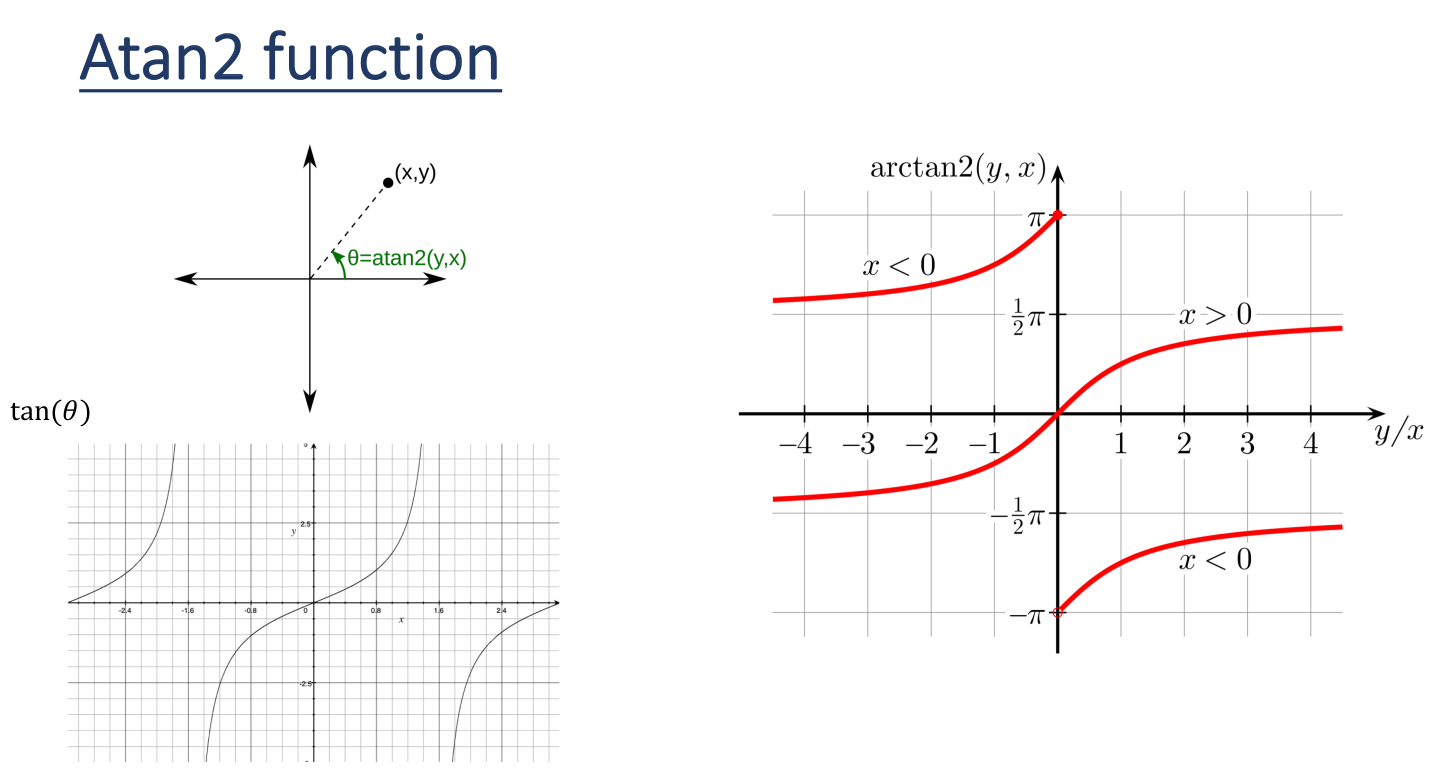
\includegraphics[scale=1.3]{atan2.png}
    \caption{atan2 - definition}
    \label{fig:sr}
    %\centering
    \end{figure}
    \end{enumerate}


 % https://en.wikipedia.org/wiki/Euler_angles
 % http://eecs.qmul.ac.uk/~gslabaugh/publications/euler.pdf

\newpage
\subsection{Angle and axis representation}
\begin{itemize}
    \item \textbf{Non0minimal representation $R(\vec{r},\; \nu )$}
    \item Unit vector $\vec{r} = (r_{x}, \; r_{y}, \; r_{z} )$
    \item Rotation angle $ \nu $ about $ \vec{r} $
\end{itemize}

\begin{figure}[h!]
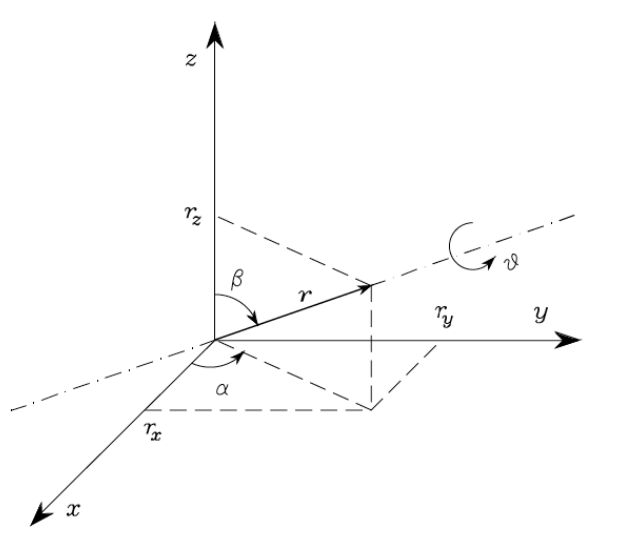
\includegraphics[scale=1.5]{axisAngle.png}
\caption{axis-angle representation}
\label{fig:sr}
%\centering
\end{figure}

\textbf{Matrix representation:}
\begin{enumerate}
    \item Alight $\vec{r} $ with $ \vec{z}  \xrightarrow[]{}  R_{y}(-\beta)R_{z}(-\alpha) $
    \item Apply $ \nu  \xrightarrow[]{}  R_{z}(\nu)$
    \item Re-aligh with $\vec{r} \xrightarrow[]{}  R_{z}(\alpha)R_{y}(\beta) $
\end{enumerate}
$$ R(\nu, r)  = R_{z}(\alpha)R_{y}(\beta)R_{z}(\nu)R_{y}(-\beta)R_{z}(-\alpha) $$
$$
R(\nu, r) =
\begin{bmatrix}
r^{2}_{x}(1-C_{\nu})+C_{\nu} & r_{x}r_{y}(1-C{\nu} ) - r_{z}S){\nu} & r_{x}r_{z}(1-C_{\nu} )+r_{y}S_{\nu} \\
r_{x}r_{y}(1-C_{\nu})+r_{z}S_{\nu} & r^{2}_{y}(1-C_{\nu})+C_{\nu} & r_{y}r_{z}(1-C_{\nu})-r_{x}S{\nu} \\
r_{x}r_{z}(1-C_{\nu})-r_{y}S_{\nu} & r_{y}r_{z}(1-C_{\nu})+r_{x}S_{\nu} & r^{2}_{z}(1-C_{\nu})+C_{\nu}
\end{bmatrix}
$$
Note: $ R(-\nu, -r) = R(\nu, r)$
While $\nu=0$ there is singularity, all $R$ matrix is zero.


\subsubsection{Inverse problem}

$$ \nu = \arccos \left(
\frac{r_{11}+r_{22}+r_{33}+1}{2}
\right)
$$
$$ r = \frac{1}{2S_{\nu}}
\begin{bmatrix}
r_{32}-r_{23}\\
r_{13}-r_{31}\\
r_{21}-r_{12}
\end{bmatrix}
, \quad for \:\: S_{\nu}\ne0
$$
for $ \nu = 0$ vertor $\vec{r}{}$ is arbitrary (singularity).

\newpage
\subsection{Quaternions}

\begin{itemize}
    \item Less intuitive than Euler/axis-angle
    \item Unique inverse
    \item No gimbal lock
    \item Fast, stable implementation
\end{itemize}

\subsubsection{2D Rotation and Complex Numbers}
\begin{itemize}
    \item Comlex number is a tuple: $a+bi$
    \item Where: $i^{2}=-1$
    \item Addition: $(a+bi)+(c+di) = (a+c) + (b+d)i$
    \item Multiply: $ (a+bi)(c+di) = ac + adi + bci +bd\cancelto{-1}{i^2} = (ac-bd)+(ad+bc)i  $
    \item Euler formula: $e^{i\theta} = ( \cos{\theta} + i\sin{\theta})$ \\
    rotation by $\theta$: \\
    $ e^{i\theta}(x+iy) = (C_{\theta}+iS_{\theta})(x+yi)=(xC_\theta-yS_{\theta} )+i(xS_\theta-yC_{\theta} ) $\\
    $$ \begin{bmatrix}
    x'\\y'
    \end{bmatrix}
    =
    \begin{bmatrix}
    C_{\theta} & -S_{\theta} \\
    S_{\theta} & C_{\theta}
    \end{bmatrix}
    \begin{bmatrix}
    x\\y
    \end{bmatrix}
    $$
    \begin{figure}[h!]
    \centering
    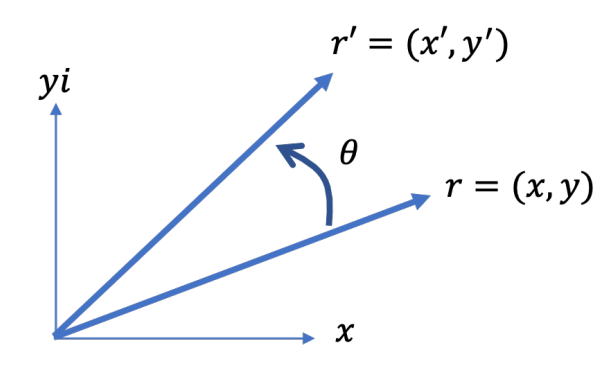
\includegraphics[scale=0.9]{complexMul.png}
    \caption{complex multiplication}
    \label{fig:sr}
    \end{figure}
    Complex multiplication=rotation(!)
\end{itemize}
\subsubsection{Quaternions}
\begin{itemize}
    \item Quaternion is a 4-tuple $ q_0 +q_1 i+ q_2 j + q_3 k $
    \item Where: \\
    \begin{figure}[h!]
    \centering
    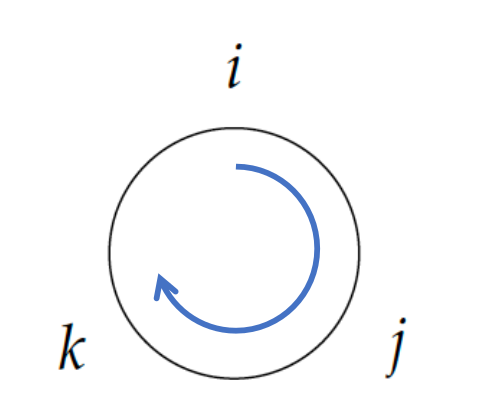
\includegraphics[scale=0.9]{quatOrder.png}
    \caption{quaternion multiplication order}
    \label{fig:sr}
    \end{figure}
    $$ i^2 = j^2 + k^2 = -1 $$
    $$ ij=k,\:\: ji=-k $$
    $$ jk=i,\:\: kj=-i $$
    $$ ki=j,\:\: ik=-j $$
    \item Addition:
    \begin{gather*}
    (q_0+q_1i+q_2j+q_3k) + (p_0+p_1i+p_2j+p_3k) = \\
    = (q_0 + p_0) + (q_1 + p_1)i + (q_2 + p_2)j + (q_3 + p_3)k
    \end{gather*}

    \item Multiplication:
    \begin{gather*}
        (q_0+q_1i+q_2j+q_3k)(p_0+p_1i+p_2j+p_3k) = \\
        = (q_0p_0 + q_1p_1i^2 + q_2p_2j^2 + q_3p_3k^2) + \\
        (q_0p_1i + q_1p_0i + q_2p_3jk + q_3p_2kj) + \\
        (q_0p_2j + q_2p_0j + q_1p_3ik + q_3p_1ki) \\
        (q_0p_3k + q_3p_0k + q_1p_2ij + q_2p_1ji) = \\
        = (q_0p_0 - q_1p_1 + q_2p_2 + q_3p_3) + \\
        (q_0p_1 + q_1p_0 + q_2p_3 - q_3p_2)i + \\
        (q_0p_2 + q_2p_0 - q_1p_3 + q_3p_1)j \\
        (q_0p_3 + q_3p_0 + q_1p_2 - q_2p_1)k
    \end{gather*}

    \item Quaternion Conjugate: \\
    \begin{gather*}
        q=q_0+Q_1i+q_2j+q_3k\\
        q*=q_0-Q_1-+q_2j-q_3k
    \end{gather*}
    \item Quaternion Norm: \\
    $ \left|q\right|=\sqrt{q^2_0+q^2_1+q^2_2+q^2_3} $
    \item Quaternion inverse:
    $ qq* = q^2_0+q^2_1+q^2_2+q^2_3 \:\: \implies (Norm)^2$
    $$q^-1 = \frac{q*}{|q|^2} $$
    \item Quaternions for rotations
    \begin{itemize}
        \item Vector $(x,y,z)$ is a pure quaternion: $0+xi+yj+zk $
        \item Rotation = Unit quaternion $q_R:|q_R|=1$
        \item Rotation from frame B to frame A:
        \begin{gather*}
         q_b = q_Rq_Aq^*_R
        \end{gather*}
        While $q_R$ is a unit quaternion\\
        $q_A \:\: q_B$ are pure quaternions.
        \begin{gather*}
            q_Rq_Aq^*_R = (q_0 + q_1i + q_2j + q_3k)(xi + yj + zk)(q_0 - q_1i - q_2j - q_3k) = \\
            (x(q^2_0 + q^2_1 - q^2_2 - q^2_3) + 2y(q_1q_2-q_0q_3)+2z(q_0q_2+q_1q_3))i + \\
            (2x(q_0q_3 + q_1q_2)+y(q^2_0 - q^2_1 + q^2_2 - q^2_3) + 2z(q_2q_3-q_0q_1))j + \\
            (2x(q_1q_3-q_0q_2)+2y(q_0q_1+q_2q_3)+z(q^2_0 - q^2_1 - q^2_2 + q^2_3))k
        \end{gather*}
        \item Matrix notation for $q_Rq_Aq^*_R$: $M\cdot(x,y,z)^T$:
        \begin{gather*}
            M =
          \begin{bmatrix}
            q^2_0 + q^2_1 - q^2_2 - q^2_3 & 2(q_1q_2-q_0q_3) & 2(q_0q_2+q_1q_3) \\
            2(q_0q_3 + q_1q_2) & q^2_0 - q^2_1 + q^2_2 - q^2_3 & 2(q_2q_3-q_0q_1)  \\
            2(q_1q_3-q_0q_2) & 2(q_0q_1+q_2q_3) & q^2_0 - q^2_1 - q^2_2 + q^2_3
          \end{bmatrix}
        \end{gather*}
        \item Simplification of $M$ matrix:
        \begin{gather*}
            M = 2\cdot
            \begin{bmatrix}
            q^2_0 + q^2_1 -0.5 & q_1q_2-q_0q_3 & q_0q_2+q_1q_3  \\
            q_0q_3 + q_1q_2 & q^2_0 + q^2_2 - 0.5 & q_2q_3-q_0q_1 \\
            q_1q_3-q_0q_2 & q_0q_1+q_2q_3 & q^2_0 + q^2_3 - 0.5
            \end{bmatrix}
        \end{gather*}
    \end{itemize}
    \item Rotation Matrix to Quaternion:
    \begin{gather*}
            R =
        \begin{bmatrix}
            r_{11} & r_{12} & r_{13} \\
            r_{21} & r_{22} & r_{23} \\
            r_{31} & r_{32} & r_{33}
        \end{bmatrix} = 2\cdot
        \begin{bmatrix}
            q^2_0 + q^2_1 -0.5 & q_1q_2-q_0q_3 & q_0q_2+q_1q_3  \\
            q_0q_3 + q_1q_2 & q^2_0 + q^2_2 - 0.5 & q_2q_3-q_0q_1 \\
            q_1q_3-q_0q_2 & q_0q_1+q_2q_3 & q^2_0 + q^2_3 - 0.5
        \end{bmatrix}
    \end{gather*}
    \begin{gather*}
        q_0 = \frac{1}{2}\sqrt{r_{11}+r_{22}+r_{33}+1} \textrm{ (We will take the positive result only)}\\
        \begin{bmatrix}
        q_1\\
        q_2\\
        q_3
        \end{bmatrix}
        =\frac{1}{2}
        \begin{bmatrix}
        sgn(r_{32}-r_{23})\sqrt{r_{11}-r_{22}-r_{33} + 1}\\
        sgn(r_{13}-r_{31})\sqrt{r_{22}-r_{33}-r_{11} + 1}\\
        sgn(r_{21}-r_{12})\sqrt{r_{33}-r_{11}-r_{22} + 1}
        \end{bmatrix}
        \textrm{, No singularity!}
    \end{gather*}
    \item Axis/Angle to Quaternion
    \begin{itemize}
        \item Scalar part: $q_0=\cos{(\nu/2)}$
        \item Vector port $(q_1,q_2,q_3) = \sin{(\nu/2)}\vec{r}{} $\\
        \begin{gather*}
           q_1 = r_x\sin{(\nu/2)} \\
           ...
        \end{gather*}
        $$ q^2_0 + q^2_1 + q^2_2 + q^2_3 = 1 $$

        \item Same quaternion for $(-\vec{r}{}, -\nu), (\vec{r}{}, \nu)$:\textbf{unique!}
        \item $\nu \in [-\pi, \pi]:q_0\geq0$
    \end{itemize}
\end{itemize}
    \subsubsection{Homogeneous Transformations}
    \begin{figure}[h!]
    \centering
    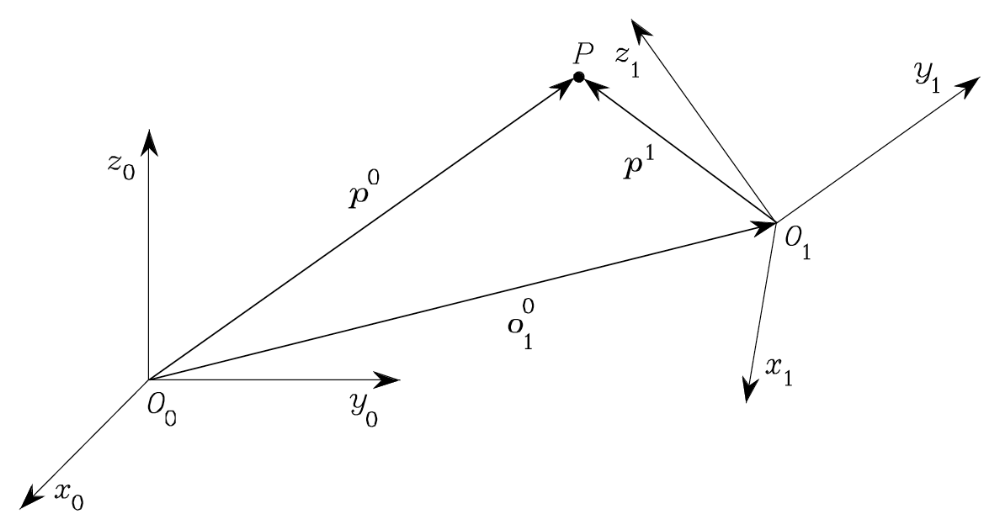
\includegraphics[scale=0.9]{homogenTr.png}
    \caption{Rotation and translation}
    \label{fig:sr}
    \end{figure}
    The normal way to do it is:
    \begin{gather*}
        p^0 = o^0_1+R^0_1p^1\\
        p^1 = -R^{0T}_1o^0_1+R^{0T}_1p^0 \:;\: R^{0T}_1 = R^1_0\\
        p^1 = -R^1_0o^0_1+R^1_0p^0
    \end{gather*}
    As you can see it is not so comfortable, so the following trick is needed:\\
    \textbf{Homogeneous}, we will define:
    \begin{gather*}
        \Tilde{p} = \begin{bmatrix}
        p\:[3\times1]\\ 1
        \end{bmatrix} \:;\:
        A^0_1 = \begin{bmatrix}
        R^0_1\:[3\times3] & o^0_1\:[3\times1] \\
        0^T \: [3\times1] & 1
        \end{bmatrix}\\
        \textrm{so the transformation can be defined as:}\\
        \Tilde{p}^0= A^0_1\Tilde{p}^1
    \end{gather*}
    \begin{gather*}
        A^0_1\Tilde{p}^1 = \begin{bmatrix}
        R^0_1 & o^0_1 \\
        0^T &1
        \end{bmatrix}
        \begin{bmatrix}
        p^1 \\ 1
        \end{bmatrix} =
        \begin{bmatrix}
        (R^0_1p^1+o^0_1) \\
        1
        \end{bmatrix} = \Tilde{p}^0
    \end{gather*}
    \\ So, all transformation is now very easy to define:
    \begin{gather*}
        \Tilde{p}^0 = A^0_1\Tilde{p}^1 \Longleftrightarrow \Tilde{p}^1 = A^1_0\Tilde{p}^0 = (A^0_1)^{-1}\Tilde{p}^0
    \end{gather*}
    \\very important to notice $A^-1\ne A^T$
    \\Using that trick we can now see a Sequence of transformations as the following:
    \begin{gather}
        \Tilde{p}^0 = A^0_1A^1_2...A^{n-1}_n\Tilde{p}^n
    \end{gather}
    $A^{i-1}_i$ : homogeneuos transformation for point in frame $i$ to the description of the same point in frame $i-1$

%\newpage
\section{Camera Calibration and 3d reconstruct}
Camera calibration is the process of estimating the parameters of camera, which affect every image no matter the camera pose in the world e.g the camera setup sensor/iris/lens. Parameters and coefficients that determine an accurate relationship between \textbf{3D point} in the real world and its corresponding \textbf{2D projection} (pixel) in the image captured by that calibrated camera.\\
Two sets of parameters:
\begin{itemize}
    \item \textbf{Intrinsic Parameters} - camera/lens system:
    \begin{itemize}
        \item Focal length (x-axis/y-axis)
        \item Optical center (center pixel, along the optical axis)
        \item Radial distortion coefficients of the lens.
    \end{itemize}
    \item \textbf{Exterinsic parameters} - orientation (rotation and translation) of the camera with respect to some world coordinate system.
\end{itemize}
\subsection{Intrinsic parameters}
$$K = \begin{bmatrix}
f_x & \gamma & c_x \\
0 & f_y & c_y \\
0 & 0 & 1
\end{bmatrix} $$\\
$f_x, f_y$ - x, y focal lengths (typically the same), in pixels or mm \\
$c_x, c_y$ - x, y coordinates of the optical axis in the image plane (pixels) \\
$\gamma$ - skew between the axes, usually 0.\\
\textbf{Some geometrical essence}
\begin{itemize}
	\item If focal lengths  $f_x, f_y$ is given in $\left[ pixels \right]$ in order to get the focal length in $\left[ mm \right]$ use the following: $f_x\left[ mm \right] = f_x\left[ pixels \right]\times pixelPitch[x]$, where, $pixelPitch[x]$ - is the physical pixel size (on the sensor), the same is for $f_y$.
	\item focal lengths  $f_x, f_y$  we can calculate the camera $\left[fov\right]$, field of view, using simple geometry.\\
	in case the focal length is given in pixels:
	$$fov_{[x]} = 2\times\arctan{\left(\frac{img_{width}\left[pixels\right]}{2\times f_x}\right)} $$
    $$fov_{[y]} = 2\times\arctan{\left(\frac{img_{height}\left[pixels\right]}{2\times f_y}\right)} $$
in case the focal length is given in mm, use sensor dimentions:
	$$fov_{[x]} = 2\times\arctan{\left(\frac{sensor_{width}\left[pixels\right]}{2\times f_x}\right)} $$
    $$fov_{[y]} = 2\times\arctan{\left(\frac{sensor_{height}\left[pixels\right]}{2\times f_y}\right)} $$   
    \item $IFOV$ - Instantaneous field of view or (IFOV) is an important calculation in determining how much a single detector pixel can see in terms of field of view (FOV).\\
    IFOV is the sapatial fov of a single pixel in an image, it is the actual image resolution in terms of angle (and if distance is known, also the actual size of a pixel in the real world), it is roughly  calculates like this, assume uniformly distributed alog the image:
    $$ifov_{[x]} = \frac{fov_x}{img_{width}[pix]} $$
    $$ifov_{[y]} = \frac{fov_y}{img_{height}[pix]} $$
    (why roughly, because in case of wide angle image (big $fov$) it is not uniformly distributed)

\end{itemize}






\newpage
\section{DH Recipe}
The DH operating recipe is as follows:
\begin{enumerate}
    \item Find and number consecutively the joint axes; set the directions of axes $z_{0}$, ...,$z_{n-1}$.
    \item Choose frame 0 by locating the
    origin on axis $z_{0}$; axes $x_{0}$ and $y_{0}$ are chosen so as to obtain a right-handed frame. If feasible, it is worth choosing frame 0 to coincide with the base frame.

Execute steps 3-5 for $n = 1,\:\dots,\: n - 1$

    \item In order to locate the origin $O_i$:
    \begin{enumerate}
        \item If axes $z_i$ and $z_{i-1}$ are parallel:
        \begin{enumerate}
            \item If joint $i$ is revolute, locate $O_i$ so that $d_i = 0$
            \item If joint $i$ is prismatic, locate $O_i$ t a reference position for the joint range, e.g., a mechanical limit.
        \end{enumerate}
        \item Otherwise, locate the origin $O_i$ at the intersection of $z_i$ with the common normal to axes $z_{i-1}$ and $z_{i}$
    \end{enumerate}
    \item Choose axis $x_{i}$along the common normal to axes $z_{i-1}$ and $z_{i}$ Pointing towards the end-effector.
    \item Choose axis $y_{i}$ so as to obtain a right-handed frame. \\
    To complete:
    \item Choose frame n:
    \begin{enumerate}
        \item If joint $n$ is revolute, align $z_{n}$with $z_{n-1}$
        \item If joint $n$ is prismatic, choose $z_{n}$ arbitrarily. \\
        Axis $x_{n}$ s set according to step 4.
    \end{enumerate}
    \item For $i = 1, ... , n$ form the table of parameters $a_i, d_i, \alpha_i, \vartheta_i$
    \item Compute the homogeneous transformation matrices $A_{i-1}^{i}$ for $i = 1, ..., n$
    \item Compute $T_{0}^{n} = A_{1}^{0}A_{2}^{1}...A_{n}^{n-1}(q_n)$
    \item Given $T_{0}^{b}$ and $T_{e}^{n}$, compute the direct kinematics function $T_{e}^{b}(q) = T_{0}^{b}T_{n}^{0}(q)T_{e}^{n}$
\end{enumerate}



\begin{table}[h!]
\begin{tabular}{|l|l|}
\hline
$a_i$      & Distance between $O_i$ and $O_{i'}$        \\ \hline
$d_i$      & Coordinade of $O_{i'}$ along $z_{i - 1}$   \\ \hline
$\alpha_i$ & \begin{tabular}[c]{@{}l@{}}Angle between axes $z_{i-1}$ and $z_i$ about axis $x_i$ to be taken\\  positive when rotation is made counterclockwise  (right handed)\end{tabular} \\ \hline
$\vartheta_i$  & \begin{tabular}[c]{@{}l@{}}Angle between axes $x_{i-1}$ and $x_i$ about axis $z_{i-1}$ to be taken\\ positive when rotation is made counterclockwise (right handed)\end{tabular}                                      \\ \hline
\end{tabular}
\\** $O_{i'}$: the intersection of the common normal to $z_{i}$ and $z_{i-1}$ with $z_{i-1}$
\end{table}


\newpage
\begin{figure}[h!]
\centering
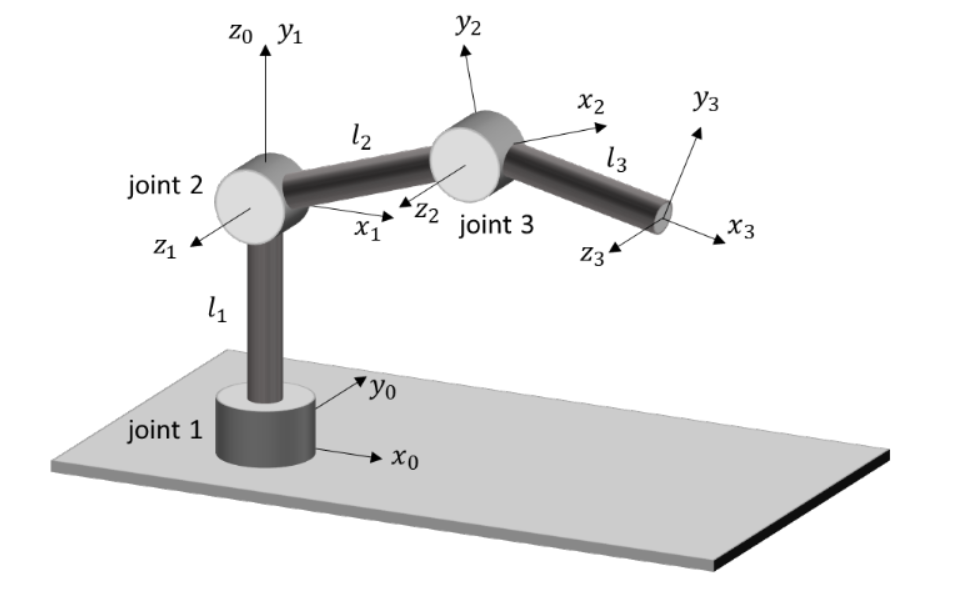
\includegraphics[scale=0.36]{roboSample.png}
\caption{sample Robot}
\label{fig:sr}
\end{figure}

\section{DH Helper}



\begin{table}[h!]
    \begin{tabular}{|l|l|l|l|l|}
        \hline
        Link & $a_i$   & $\alpha_i$ & $d_i$  & $\vartheta_i$ \\ \hline
        $1$  &  $0$    &    $\pi/2$ &  $l_1$ & $\vartheta_1$ \\ \hline
        $2$  &  $l_1$  &    $0$     &  $0$   & $\vartheta_2$ \\ \hline
        $3$  &  $l_2$  &    $0$     &  $0$   & $\vartheta_3$ \\ \hline
\end{tabular}
\end{table}

Each line on the table is transformed to that matrix:

    \begin{equation*}
        \begin{bmatrix}
        C\vartheta_i &  -S\vartheta_i C\alpha_i &  S\vartheta_i S\alpha_i &  a_i C\vartheta_i\\
        S\vartheta_i & C\vartheta_i C\alpha_i   & -C\vartheta_i S\alpha_i & a_i S\vartheta_i \\
        0            & S\alpha_i                & C\alpha_i               & d_i              \\
        0            & 0                        & 0                       & 1
        \end{bmatrix}
    \end{equation*}


\begin{enumerate}
    \item Link $l_i$ is between $O_{i-1}$ and  $O_{i}$
    \item The lines $_i$ on D-H table are per \textbf{link!}
    \item Common normal is between $z_{i-1}$ and $z_{i}$ (right handed),

\end{enumerate}


\end{document}
